\documentclass [a4paper,12pt]{article}
\usepackage{url}
\usepackage{xcolor}
\usepackage{listings}
\usepackage{amssymb}
\usepackage{amsfonts}
\usepackage{graphicx}
\usepackage{caption}
\usepackage{subcaption}
\usepackage{units}
\usepackage{fullpage}

\include{listing_style}
\def \fftw {\texttt{fftw}}
\def \lmvn {\texttt{libmultiviewnative}}
\def \cufft {\texttt{cufft}}
\def \gpu {GPGPU}
\def \cpu {CPU}

\title{Streaming FFTs on large 3D microscope image data}
\author{Peter Steinbach, MPI CBG}
%\institute{MPI CBG}
\begin{document}
\maketitle
\begin{abstract}

\end{abstract}

\section{Introduction}

Light sheet microscopy today has become the hallmark experimental technique of systems biology \cite{Huisken13082004, Keller14112008}. It allows image aquisition of large alive developing specimens, high temporal and spatial resolution, imaging from multiple angles as well as low photodamage to the specimen which enables long timelapse recordings. However, due to the limited optical performance of the used equipment and the constant tradeoff between acquisition frequency and resolution, segmenting the produced data for further analysis is challenging. Deconvolution is the operation of restoring spatial resolution and contrast of this data given the knowledge of the underlying optics after the imagery has been recorded. Here, Selective Plane Illumination Microscopy (SPIM) data offers high potentials for SPIM records the same geometric location from different angles.\newline

The authors of \cite{2013arXiv1308.0730P} have provided an optimized formulation of the iterative expectation-maximization algorithm used to deconvolve SPIM data. This implementation thereof \cite{gh_spim_registration} is the starting point for this study whose motivation is to further increase performance and turnover of the algorithm by porting it entirely to run on General Purpose Graphics Processing Units (GPGPUs) using the CUDA programming platform \cite{Nickolls:2008:CUDA}. The implementation is available as a free and open-source library from \cite{lmvn_repo}.\newline

For the purpose of this paper, the subsequent discussion will first discuss the current algorithm implementation and common usage patterns(section \ref{sec:alg}), followed by a brief description of the benchmark hardware (section \ref{sec:hw}). The focus of the paper will then be on developing a performant implementation through a bottoms-up approach using model implementations (section \ref{sec:models}), before concluding with a summary and outlook (section \ref{sec:summ}).\newline

\section{Algorithm Details and Usage}
\label{sec:alg}
Given the recorded SPIM observations $\phi_\nu$ of a geometric volume for each angle $\nu$ (also referred to as \textit{view}), the current deconvolved estimate $\psi^{r+1}$ for iteration $r+1$ is given by (in a very general form):\newline

\begin{equation}
\psi^{r+1} = \psi^{r} \prod_{\nu \in V} \frac{\phi_{\nu}}{\psi^{r} \ast P_{\nu} } \ast P^{compound}_{\nu}
\label{iterative_deconv}
\end{equation}

Here, $P_{\nu}$ refers to the experimentally obtained optical point-spread function (PSF) for angle $\nu$. $\ast$ denotes the discrete convolution, i.e. given an image $f$ and a convolution kernel $g$ the convolution of the two would be given by $f \ast g$. $P^{compound}_{\nu}$ denotes a compound point spread function over virtual views calculated from all $P_{\nu}$. The interested reader is hereby referred to \cite{2013arXiv1308.0730P} for the derivation and further details that lead to and explain equation \ref{iterative_deconv}.\newline

The implementation of the above was performed in java \cite{fiji_wiki_mvd} and is available as a plugin to the fiji image analysis platform \cite{fiji_website}. The core algorithm can be described in pseudo-code as in listing \ref{lst:java_implementation}.\newline

\begin{lstlisting}[caption={Java Implementation of Multi-View Deconvolution.},label={lst:java_implementation}]
stack_f32 psi = stack_f32(const);
stack_f32 view[n_view], kernel1[n_view],     //loaded from disk
	  kernel2[n_view], weights[n_view];  //loaded from disk

for( i : n_iterations ){
  for( v : n_view ){
    stack_f32 temp = psi;
    temp = convolve(temp,kernel1[v]);	    
    temp = view[v]/temp;
    temp = convolve(temp,kernel2[v]);	    
    psi = regularize(psi, temp, weights);
  }
}
\end{lstlisting}

In listing \ref{lst:java_implementation}, \texttt{stack\_f32} refers to a type that describes a three dimensional image where each intensity is encoded as a 32-bit floating point number. Related to this, the C/C++ array notation is used to indicate that each run of the deconvolution requires all image views \texttt{stack\_f32 view[n\_view]}, all per-view PSFs \texttt{kernel1[n\_view]}, all compound PSFs \texttt{kernel2[n\_view]} and all weight distributions \texttt{weights[n\_view]} to be available in memory. \texttt{psi} notes the deconvolved view that is updated by each iteration of the double loop in line $4-5$. The function call \texttt{convolve} denotes the convolution described in equation \ref{iterative_deconv} as $\ast$. The regularization mentioned in listing \ref{lst:java_implementation} has been omitted from equation \ref{iterative_deconv} for the sake of clearity, but is further described in the corresponding paper \cite{2013arXiv1308.0730P}. Any padding to the input \texttt{view} and \texttt{weights} as well as embedding of both PSFs into zero-filled images of same shape as \texttt{view} is omitted from listing \ref{lst:java_implementation} for readability. \newline

\begin{table}
  \begin{tabular}{ccc}                                                                                                                                                                              
    \hline                                                                                                                                                                                         
    View Shape  & Number of Views and Channels & Data Volume [MB]   \\
    \hline                                                       
    $928\times390\times390$ & $6 \times 1$ & $807$ \\
    $1670\times1070\times345$ & $4 \times 2$ & $4703$ \\
    \hline                                                                                                                                                                                         
  \end{tabular} 
  \label{typ_datasets}
  \caption{Typical SPIM datasets dimensionality, number of views and color channels (per view). All datasets save the pixel intensity as 16-bit integer value. The latter has been used to calculate the raw data set volume.}
\end{table} 

In order to set the implementation to scale, table \ref{typ_datasets} lists typical data sets from SPIM instruments. It is important to note that the majority of instruments store the image data as 16-bit integer value. Typical sizes of the PSF are on the order of $23 \times 81 \times 85$. \\

As the algorithm at hand relies twice on convolutions, this operation is deemed to be the largest consumer of run time. A convolution is a filtering operation, that operates on and n-dimensional image $f$ and convolves it by a filter kernel $g$ of similar or less dimensionality. Assuming that $f$ and $g$ are three-dimensional pixel collections and that $g$ has dimensions $N_{x} \times N_{y} \times N_{z}$, a convolution for an output pixel at location $[x,y,z]$ is calculated as 

\begin{equation}
  \label{eq:disc_convolve}
  (f \ast g)[x,y,z] = \sum^{i_x = N_{x}/2}_{i_x = -N_{x}/2} \sum^{i_y = N_{y}/2}_{i_y = -N_{y}/2} \sum^{i_z = N_{z}/2}_{i_z = -N_{z}/2} f[x-i_x,y-i_y,z-i_z] \cdot g[i_x,i_y,i_z].
\end{equation}

This operation does not only yield complications towards the borders of $f$ where $f[x-i_x,\dots]$ may refer to a pixel location outside the actual image (i.e. of unknown intensity), it is moreover of complexity 

\begin{equation}
\label{eq:discrete_convol_complexity}
\mathcal{O}(F[f \ast g]) = \mathcal{O}(I_{x} I_{y} I_{z} N_{x} N_{y} N_{z})
\end{equation}


where $I_{n}$ refers to the extent of $f$ in dimension $n$. Given the datasets listed in table \ref{typ_datasets}, this is an computationally expensive operation. As the convolution per output pixel $(f \ast g)[x,y,z]$ is independent of the calculation of every other output pixel $(f \ast g)[x',y',z']$, a convolution might at first glance yield high speed-ups when implemented on GPGPUs. As discussed in \cite{eklund_nonseparable_filtering}, this is only true for small kernel sizes on the order of $6 \times 6 \times 6$ at a fixed input image size. This is due to the fact that 2 arithmetic operations for every 2 arithmetic operations have to be performed. This results in an arithmetic complexity (number of arithmetic operations divided by the number of memory loads) of $1$. This has long been known \cite{massively_parallel_book} to be a regime, where GPGPUs do not perform well. To mitigate this short coming, the convolution theorem (equation \ref{}) can be exploited which states that a convolution in the spatial domain can be performed as a multiplication in the frequency domain.

\begin{equation}
  \label{eq:convol_theorem}
  F[f \ast g] = F[f] \cdot F[g]
\end{equation}

Here, $F[f]$ gives the Fourier Transform of $f$ into the frequency domain and $\cdot$ notes the element-wise multiplication of $F[f]$ and $F[g]$. The implementation of fast Fourier Transforms (FFT) has been studied for more than 50 years by now \cite{FFTCooleyTurkey,FFTBluestein,FFTRaders}. For the purpose of convolution, the complexity of the algorithm is hence reduced to 

\begin{equation}
  \label{eq:fft_convol_complexity}
  \mathcal{O}(F[f] \cdot F[g]) = 2\times\mathcal{O}(I\log I) + \mathcal{O}(I) = \mathcal{O}(I\log I)
\end{equation}

Here, $I = I_{x} \cdot I_{y} \cdot I_{z}$ refers to the total number of pixels in image $f$. As the FFT is performed on non-complex data further simplifications can be applied to it's implementation which renders equation \ref{eq:fft_convol_complexity} to be an upper bound rather than an exact value as in equation \ref{eq:discrete_convol_complexity}. The library as the result of the discussion at hand interfaces to the \texttt{fftw} (\cite{FFTW05}) library which contains highly optimised FFT implementations performed on the Central Processing Unit (CPU). The CPU-based implementation of the multi-view deconvolution is based on listing \ref{new_implementation}.

\begin{lstlisting}[caption={Optimized CPU Implementation of Multi-View Deconvolution. All FFT are explicitely stated \texttt{fft} as well as the corresponding normalized inverse operations \texttt{ifft}. },label={lst:new_implementation}]
stack_f32 psi = stack_f32(const);
stack_f32 view[n_view], kernel1[n_view],     //loaded from disk
	  kernel2[n_view], weights[n_view];  //loaded from disk

for( v : n_view ){
  kernel1[v] = fft(kernel1[v]);
  kernel2[v] = fft(kernel2[v]);
}

for( i : n_iterations ){
  for( v : n_view ){
    stack_f32 temp = psi;
    temp = ifft(fft(temp)*kernel1[v]);
    temp = view[v]/temp;
    temp = ifft(fft(temp)*kernel2[v]);
    psi = regularize(psi, temp, weights);
  }
}
\end{lstlisting}

Listing \ref{lst:new_implementation} contains one central improvement over listing \ref{lst:java_implementation}, whereby the FFT of \texttt{kernel1} and \texttt{kernel2} is performed before the iterative double loop is entered. This removes $n_{iterations}\cdot n_{view}$ executions of a FFT of size $I$ from the algorithm, which is beneficial not only in terms of runtime but also in terms of the memory budget.

For the GPGPU implementation interfacing to the \texttt{cufft} library (\cite{cufft}), the CPU implementation is used as a reference for code validation.


\clearpage
\section{Hardware}
\label{sec:hw}

For the measurements at hand, a Dell T7810 work station was used equipped with two Intel Xeon E5-2540 v3 processors and $\unit[64]{GB}$ of DDR4-2133 RAM. The workstation supported a Nvidia Tesla K20c provided by the TU Dresden based CUDA Center Of Excellence. The operating system was CentOS 7. To broaden the scope, a passively cooled Nvidia Tesla M2090 operated inside a rack-mounted Dell C6100 with two Intel Xeon E5-2640 and $\unit[128]{GB}$ of RAM. The operating system was CentOS 6.3 and all compilations were performed with gcc 4.8.3 and cuda 6.5. All compilations were performed with gcc 4.8.3 and cuda 6.5.14 except stated otherwise. Third, a second Dell T7810 work station with 2 Intel Xeon E5-2670 (Hyperthreading enabled), $\unit[64]{GB}$ of DDR4-2133 RAM and a Nvidia GeForce GTX Titan Black running CentOS 6.6 was included in the tests.

\section{Model}
\label{sec:models}

As shown in section \ref{sec:alg}, multi-view deconvolution relies on 3D image stack convolutions with large kernels. In order to iterate towards an efficient design of multi-view deconvolution, this section will discuss model implementations and their benchmarks on hardware introduced in section \ref{sec:hw}. All of the model systems use synthetic data which is validated after each run upon consistency where appropriate. If not stated otherwise, the synthetic data has been generated in steps of powers of 2 in each dimension, so that each benchmark was run on $64x64x64$, $128x64x64$, $128x128x64$, \dots, $1024x1024x1024$ shaped datasets if possible.

\subsection{Single FFT}

As the heart of the application are FFT, there performance on CPU and GPU should be compared. For this, the most simple setup is used.

\begin{lstlisting}[caption={Single FFT on synthetic data performed on CPU in pseudo-code based on the \fftw{} syntax.},label={lst:single_fft_cpu}]
stack_f32 synthetic_data;

fftwf_plan plan = fftw_plan_dft_r2c(3,
                                    synthetic_data.shape(),
                                    synthetic_data.ptr(),
                                    synthetic_data.ptr(),
                                    FFTW_MEASURE);
//start timing
fftwf_execute(plan)
//end timing
\end{lstlisting}

Listing \ref{lst:single_fft_cpu} gives an overview on the syntax required to execute a \fftw{} 3D FFT on spatial domain data and whose result is written back to the same memory location in the frequency domain (in-place transform). The application programming interface (API) requires plan to perform the transform operation. According to the documentation \cite{fftw_manual}, the plan allocates additional memory for structures required during FFT execution. This global variable hence exerts a software design force on all clients to be aware of this behavior. Moreover, plans should be reused in order to prevent unnecessary reallocations. The equivalent implementation to perform the FFT on the \gpu{} is given in listing \ref{lst:single_fft_gpu}.\newline

\begin{lstlisting}[caption={Single FFT on synthetic data performed on GPU in pseudo-code based on the \cufft{} syntax.},label={lst:single_fft_gpu}]
stack_f32 synthetic_data;
float* device_ptr = 0;
cudaMalloc(device_ptr, sizeof(float)*synthetic_data.size());
cudaMemcpy(device_ptr, synthetic_data.ptr() , sizeof(float)*synthetic_data.size(), cudaHostToDevice);

cufftHandle plan;
cufftPlan3d(&plan,synthetic_data.shape(0),synthetic_data.shape(1),synthetic_data.shape(2),CUFFT_R2C);

//start timing
cufftExecR2C(plan, device_ptr, device_ptr);
//end timing

cudaMemcpy(synthetic_data.ptr(), device_ptr , sizeof(float)*synthetic_data.size(), cudaDeviceToHost);
\end{lstlisting}

Clearly, the offload model of having \gpu{} memory being separate from \cpu{} memory requires a lot more syntax than for plain \cpu{} use cases. However, the \cufft{} API is similar in nature to \fftw{} except the more stringent procedural approach (no functions with return values, rather than functions operating on structs). As \texttt{cudaMemcpy} is used to transfer data from host to device and back, this implementation is internally synchronized.\newline

\begin{figure}[h]
  \centering
  \hfill
  \begin{subfigure}[b]{0.45\textwidth}
    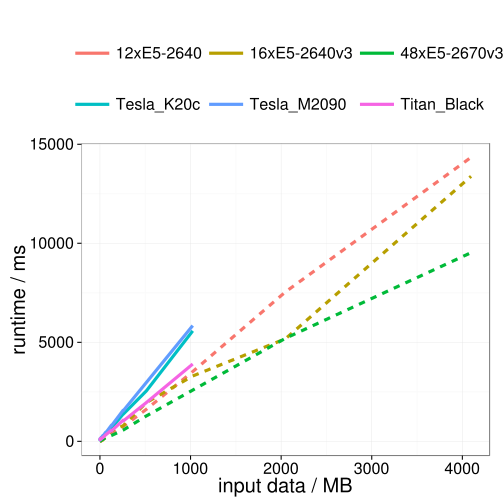
\includegraphics[width=\textwidth]{plots/synced_gpu_runtime}
    \caption{CUDA runtime}
    \label{fig:single_fft_runtime}
  \end{subfigure}%
  \hfill
  \begin{subfigure}[b]{0.45\textwidth}
    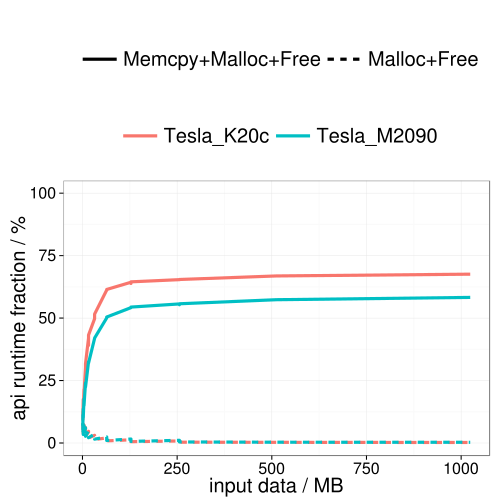
\includegraphics[width=\textwidth]{plots/synced_gpu_api_fraction}
    \caption{CUDA API fraction}
    \label{fig:single_fft_api_fraction}
  \end{subfigure}
  \hfill
  \caption{Runtimes for single 3D FFT on synthetic data on \cpu{} with \fftw{} and on \gpu{} with \cufft{} (left, \ref{fig:single_fft_runtime}) and API time fraction of runtime dedicated to data (de-)allocation and/or data transfer (right, \ref{fig:single_fft_api_fraction}).}
  \label{fig:rt_single_fft}
\end{figure}

Figure \ref{fig:rt_single_fft} illustrates the runtime budget of an FFT transformation for different input data performed on multi-core \cpu{}s or on \gpu{}s. Subfigure \ref{fig:single_fft_runtime} shows a linear rise in runtime with increasing size of input data. This is the behaviour expected from considerations of equation \ref{eq:fft_convol_complexity}. Due to the larger memory available on \cpu{}s, they are able to handle bigger data sets than \gpu{}s.\\

For the execution on a \gpu{}, it is interesting to observe what fraction of this runtime is invested in data transfers. Figure \ref{fig:single_fft_api_fraction} hints to $\unit[50-70]{\%}$ of the total runtime is dedicated to data transfers. It is interesting to see how the \gpu{} that supports PCI Express Gen3 clearly dedicates less time to memory transfers than the other modesl. \\

The API fraction measurements have been performed with \texttt{nvprof} called as in:\newline
\begin{center}
  \texttt{nvprof --normalized-time-unit ms --print-gpu-summary --print-api-summary --print-summary --profile-from-start off}\newline
\end{center}

Firgure \ref{fig:single_fft_api_fraction} implies, that if data transfer can be hidden or accelerated, this would be beneficial for the \gpu{} based algorithm to accelerate in comparions to the \cpu{} implementation.

\clearpage
\subsection{Batched FFTs}
As the transform of a single data volume is of minimal use for the application at hand, the next step is to study the transform of a sequence of image stacks with fixed sizes. In all of the following figures and discussions, 8 image stacks were used per experiment and shape configuration.\\newline
 
\begin{lstlisting}[caption={Batched FFT on synthetic data performed on CPU in pseudo-code based on the \fftw{} syntax.},label={lst:batched_fft_cpu}]
stack_f32 synthetic_data[n_view];

fftwf_plan plan = fftw_plan_dft_r2c(3,
                                    synthetic_data[0].shape(),
                                    synthetic_data[0].ptr(),
                                    synthetic_data[0].ptr(),
                                    FFTW_MEASURE);
//start timing
for ( v : n_view )
  fftwf_execute_dft_r2c(plan, 
                        synthetic_data[v].ptr(),
                        synthetic_data[v].ptr());
//end timing
\end{lstlisting}

As listing \ref{lst:batched_fft_cpu} illustrates, plan reuse is performed and \fftw{} is called with the \texttt{FFTW\_MEASURE}. During plan creation, the \fftw{} library tries to find the best FFT implementation for the given buffer shape. \texttt{FFTW\_MEASURE} guarantees a next-to-optimal solution. The GPU implementation at this point already requires a complex orchestration of memory transfer streams and execution.

\begin{figure}[h]
  \centering

  \begin{subfigure}[b]{0.9\textwidth}
    \includegraphics[width=\textwidth]{img/bench_gpu_many_nd_fft_sync_narrow}
    \caption{synchronized transform}
    \label{fig:batched_fft_sync}
  \end{subfigure}%

  \begin{subfigure}[b]{0.9\textwidth}
    \includegraphics[width=\textwidth]{img/bench_gpu_many_nd_fft_async_narrow}
    \caption{asynchronous transform}
    \label{fig:batched_fft_async}
  \end{subfigure}%

  \begin{subfigure}[b]{0.9\textwidth}
    \includegraphics[width=\textwidth]{img/bench_gpu_many_nd_fft_async2plans_narrow}
    \caption{asynchronous transform with 2 streams}
    \label{fig:batched_fft_async2plans}
  \end{subfigure}%

  \caption{\texttt{nvprof} screenshot of batched FFT transforms.}
  \label{fig:nvprof_batched_fft}
\end{figure}

Figure \ref{fig:nvprof_batched_fft} illustrates possible advantages and disadvantages of the applied techniques. As the documentation of the corresponding code for figure \ref{fig:nvprof_batched_fft} would be rather long, the interested reader is deferred to \texttt{bench\_gpu\_many\_nd\_fft.cu} of the \lmvn{} benchmark suite available through \cite{lmvn_repo}. 

\begin{lstlisting}[caption={Asynchronous Batched FFT on synthetic data performed on GPU in pseudo-code based on the \cufft{} syntax.},label={lst:batched_fft_gpu_async2plans}]
stack_f32 synthetic_data[n_view];
cudaEvent_t stream_events[n_view];
fftwf_plan plans[2];
cudaStream_t streams[2];
float* d_buffer[2];
// ... initialize 

//start timing
for ( v : n_view ){
  cudaMemcpyAsync(synthetic_data[v] -> d_buffer[v \% 2],streams[v \% 2]);
  cudaEventRecord(stream_events[v],streams[v \% 2]);
  cudaStreamWaitEvent(streams[v \% 2],stream_events[v - 1]);
  cufftExecR2C(plans[v \% 2], d_buffer[v \% 2]) // on stream d_buffer[v \% 2]
  cudaMemcpyAsync(d_buffer[v \% 2] -> synthetic_data[v],streams[v \% 2]);
}
cudaDeviceSynchronize();
//end timing

//clean-up
\end{lstlisting}


What however becomes clear is that synchronous (figure \ref{fig:batched_fft_sync}) are not beneficial as data transfers to the \gpu{} are performed sequentially. Asynchronous transfers using the same number of streams as there are image stacks (figure \ref{fig:batched_fft_async}) are also not performant (mostly due to the lack of copy engines). But if the number of transfer streams correlates with the number of copy engines the \gpu{} offers, data transfers and computations can be overlaid to some higher extent and runtime benefits can be obtained (figure \ref{fig:batched_fft_async2plans}). Besides the ones just discussed, other host-device data transfer methods were benchmarked. 
For example, mapped memory usage (buffers are marked by \texttt{cudaHostRegister} and their device pointer is obtained through \texttt{cudaHostGetDevicePointer}) and managed unified memory (all data is allocated by \texttt{cudaMallocManaged}) have been implemented. The results for ``managed'' and ``mapped'' memory usage are not shown here because time measurements did not correlated at all with the measurements obtained in \texttt{nvprof}. Before drawing wrong conclusions from an illposed measurement, the data is not discussed. 

\begin{figure}[h]
  \centering
  \hfill
  \begin{subfigure}[b]{0.45\textwidth}
    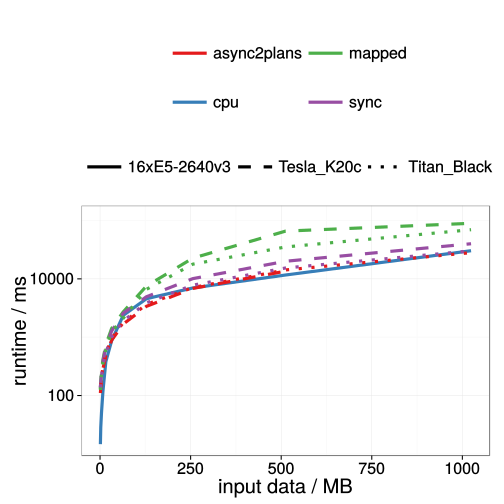
\includegraphics[width=\textwidth]{plots/batched_cgpu_runtime}
    \caption{CUDA runtime}
    \label{fig:batched_fft_runtime}
  \end{subfigure}%
  \hfill
  \begin{subfigure}[b]{0.45\textwidth}
    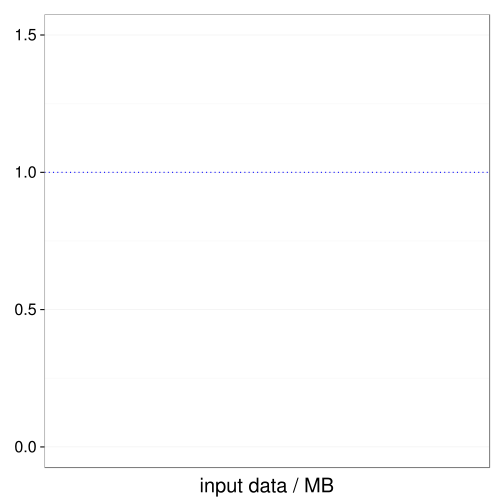
\includegraphics[width=\textwidth]{plots/batched_gpu_speed_up}
    \caption{\gpu{} speed-up versus \cpu{}}
    \label{fig:batched_fft_speed_up}
  \end{subfigure}
  \hfill
  \caption{Runtimes for 3D FFT transforms on a batch of 8 buffers from synthetic data. The results are compared to the \cpu{} implementation with \fftw{} and on the \gpu{} with \cufft{} (left, \ref{fig:single_fft_runtime}) and the relative speed-up of the \gpu{} implementation (see figure \ref{fig:batched_fft_async2plans}) compared to the multi-core \cpu{} implementation (right, \ref{fig:batched_fft_speed_up}) for different \gpu{} models.}
  \label{fig:rt_batched_fft}
\end{figure}


The synchronized implementation in figure \ref{fig:rt_batched_fft} is on par with the \cpu{} implementation for a wide range of data volumes. The differences between results from the ``K20c'' and the ``Titan Black'' \gpu{} re-confirms earlier findings from figure \ref{fig:single_fft_api_fraction}. The implementation with \texttt{cufftPlanMany} is also show and clearly breaks down with smaller image stack sizes due to \gpu{} memory constraints. The reason for this lies in the fact that \texttt{cufftPlanMany} requires all input data to be present on the \gpu{}.\\
 
The implementation referred to as ``async2plans'' in figure \ref{fig:rt_batched_fft} notes the results of listing \ref{lst:batched_fft_gpu_async2plans} in practise. Given an input data volume of $\unit[50-250]{MB}$, this implementation is faster than the \cpu{} implementation, but does not attain results above a certain data volume compared to e.g. the ``sync'' method. This is due to the fact that it requires device memory of the size of 2 input stacks as well as the workarea for two FFT transforms. This of course depends on the \gpu{} model as to what amount of device memory is available. % This is due to the fact that both the GeForce Titan Black and the Tesla M2090 do only contain 1 copy engine. The device is henceforth forced to serialize asynchronous data transfers and kernel execution.
\newline

For large data sets, the real-to-complex FFT transform performed on a \gpu{} appears not to supersede the performance of \cpu{} based implementations by a large amount. As for larger memory transfers, the time per transfer increases dramatically over the time needed for FFT relevant computations, this effect can be attributed to the PCI Express bus bandwidth and speed. Thus, the performance of ``sync'' and ``planmany'' implementations in figure \ref{fig:rt_batched_fft} must exhibit a similar behavior.

\clearpage
\subsection{Batched Convolutions}

The next level of discussing the performance of multi-view deconvolution is to look at batched 3D image convolutions. Synthetic data was used again to make up 8 training data sets, all of which were convolve with a filter kernel of size $21 \times 21 \times 21$.\\newline 


\clearpage
\subsection{Library Implementation}



\clearpage

\section{Summary}
\label{sec:summ}

Multiview Deconvolution is a central technique for contrast enhancements of multi-dimensional SPIM data. As the data is of unprecedented size, porting suche an algorithm onto massively parallel hardware (\gpu{}s) requires a constant struggle against data transfer bottlenecks. As such, the PCI Express is the everlasting hurdle to overcome by asynchronous orchestration of memory transfers to the \gpu{} and computing calls. In this study, performance considerations for model systems very similar to the environment of \lmvn{} lead to an improvement of the actual algorithm and a speed-up of $7x$ compared to a state-of-the-art multi-\cpu{} implementation.\newline


\section{Acknowledgements}
\label{sec:ackn}

I'd like to thank Stephan Preibisch (Janelia Farm) and Pavel Tomanck (MPI CBG) for providing me this challenging project that lead me to present at an internationally renowned conference. I'd also like to thank Stephan Janosch for providing test data sets and the CUDA Center of Excellence for providing the Nvidia Tesla K20c used for the experiments above as well as valuable feedback during this project. 

\section{References}
\bibliographystyle{ieeetr}
\bibliography{lmvn}
\end{document}
